% This text is proprietary.
% It's a part of presentation made by myself.
% It may not used commercial.
% The noncommercial use such as private and study is free
% Dec 2007
% Author: Sascha Frank 
% University Freiburg 
% www.informatik.uni-freiburg.de/~frank/
%
% 
\documentclass{beamer}
\setbeamertemplate{navigation symbols}{}
\usetheme{Warsaw}

\usepackage[export]{adjustbox}

\usepackage[thinlines]{easytable}

\beamersetuncovermixins{\opaqueness<1>{25}}{\opaqueness<2->{15}}

\def\mydot{\structure{\rule{1ex}{1ex}}\,}
\def\B#1{\mathbf{#1}}
\def\emph#1{\textbf{\textcolor{orange}{#1}}}
\DeclareMathOperator{\argmin}{argmin}
\DeclareMathOperator{\prox}{prox}
\DeclareMathOperator{\proj}{proj}

\newcommand{\mycite}[1]{\textcolor{myblue}{[#1]}}

%% put page number in slide footer
\newcommand*\oldmacro{}%
\let\oldmacro\insertshorttitle%
\renewcommand*\insertshorttitle{%
  \oldmacro\hfill%
  \insertframenumber\,/\,\inserttotalframenumber}

\definecolor{darkgreen}{rgb}{0,0.5,0}
\definecolor{myblue}{RGB}{102,153,255}
\definecolor{mygray}{RGB}{200,200,200}

\begin{document}

\setbeamertemplate{caption}{\raggedright\insertcaption\par}
\setlength\abovecaptionskip{-2pt}

\title{Understanding inter-subject functional variability}  
\author{Elvis Dohmatob\\ (Supervised by B. Thirion and G. Varoquaux)}
\date{\today} 


\begin{frame}
\titlepage
\end{frame}

  \setcounter{tocdepth}{1}

\begin{frame}\frametitle{Table of contents}\tableofcontents
\end{frame} 

\section{Introduction} 
\begin{frame}\frametitle{Context}
  \mydot A major goal of human neuroscience is understand
  \begin{itemize}
  \item the structure,
  \item function, and
  \item variability of the human brain
  \end{itemize}

  \uncover<2->{
    \mydot We will focus on \textbf{\textcolor{blue}{inter-subject functional variability}}
  }
\end{frame}

\subsection{Brain and functional networks}
\begin{frame}\frametitle{Brain function arises from networks}
    \centering
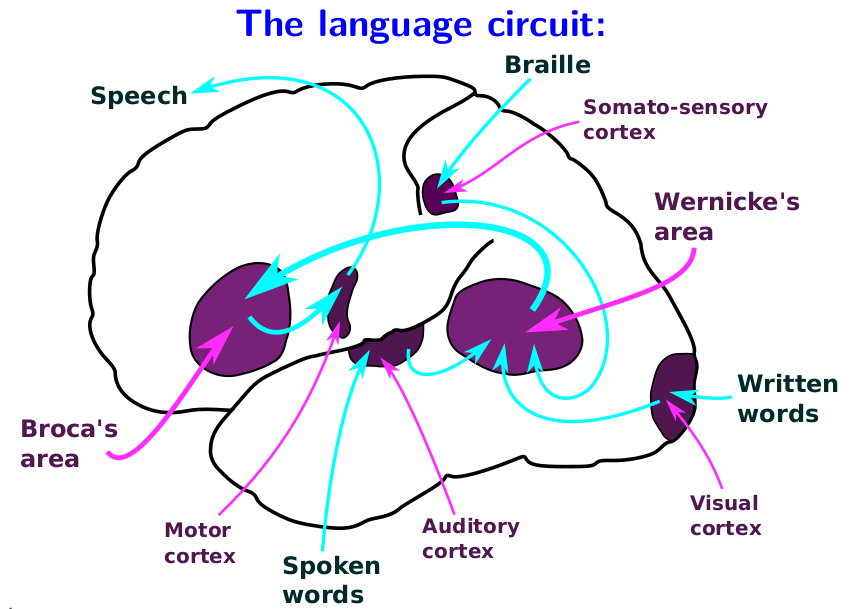
\includegraphics[scale=.3]{howbrainworks0} 

\tiny{\textit{(Courtesy of Gael Varoquaux)}}
\end{frame}


\subsection{Modalities}
\begin{frame}\frametitle{How fMRI data is acquired}
    \centering
    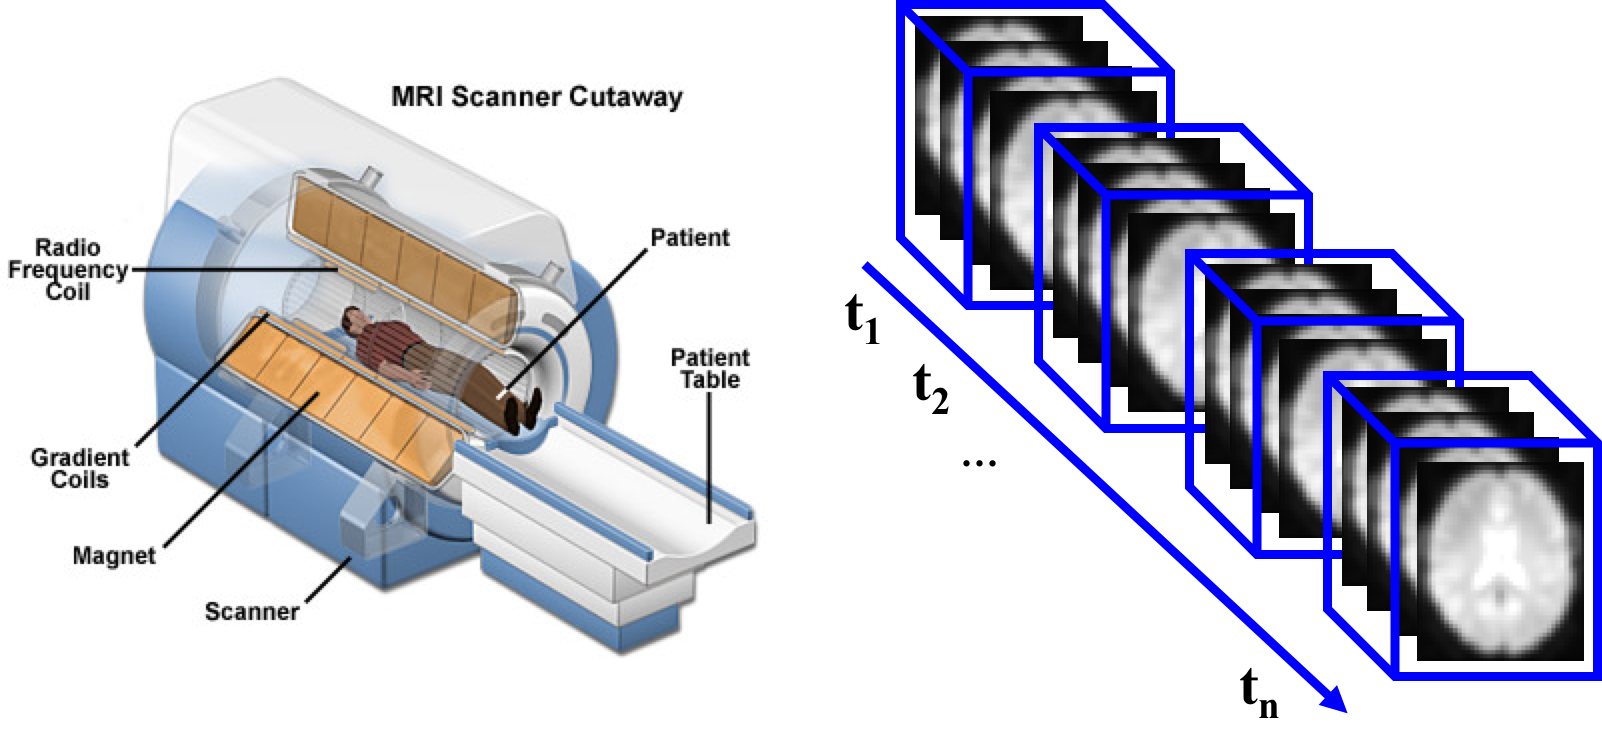
\includegraphics[scale=.4]{fmri_setup}

\tiny{\textit{(Courtesy of ???)}}
\end{frame}


\section{Structured penalties for multi-variate brain-decoding}
\subsection{Preliminaries}

\begin{frame}\frametitle{Masking}
  \centering
  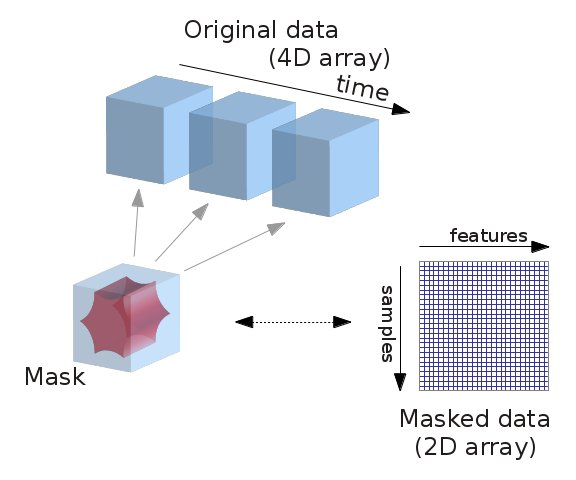
\includegraphics[width=.7\linewidth]{masking.jpg}

\mydot Each sample 3D image $\iff$ vector in $\mathbb R^p$% (via mask).
  
\end{frame}

\begin{frame}\frametitle{A zoom on  brain-decoding (supervised ML)}
    \begin{overprint}
      \only<1>{
        
        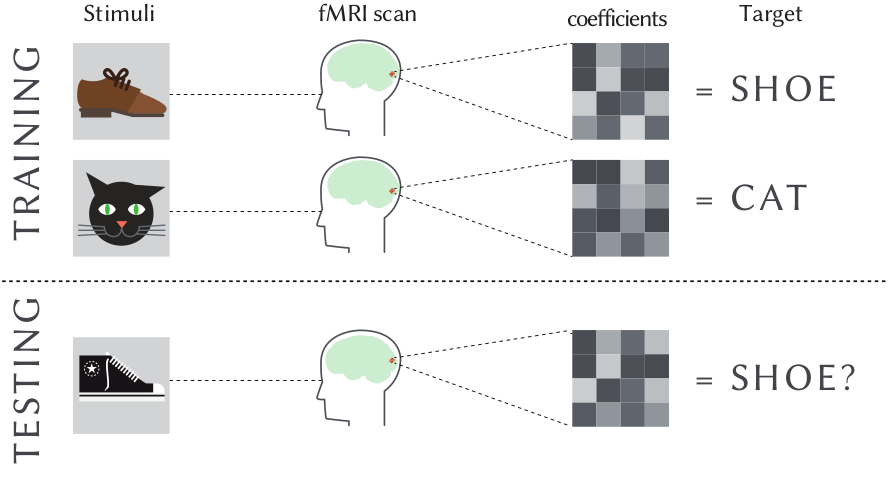
\includegraphics[width=1.\linewidth]{decoding.png}
        
    \quad\quad\quad\quad\quad\quad\quad\quad\quad\quad\quad\;\;$\bf{X}$
    \quad\quad\quad\quad\quad\quad\;\;$\bf{w}$
    \quad\quad\quad\quad\quad$\bf{y}$
  }
  
  \only<2>{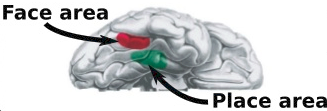
\includegraphics[width=1.\linewidth]{takehome.png}

    \mydot We don't just want good predictions, we want \emph{regions}
    }
  \end{overprint}

% \mydot \emph{$\B{X}_i$}: each sample is a 3D MRI brain image scanned at a particular instant $i$.

% \mydot \emph{$\B{y}_i$}: target, the class of the stimulus at instant $i$.

% \mydot There are as many features as voxels (up to \textcolor{red}{$10^6$}).
\end{frame}

\begin{frame}\frametitle{What we mean by ``structured''}
  \begin{overlayarea}{\textwidth}{\textheight}
\begin{columns}
  \begin{column}{7.5cm}
  \emph{Definition:}
  \begin{itemize}
  \item Localized activation patterns -- \emph{sparsity}
  \item Clusters of active voxels -- \emph{smoothness}
  \end{itemize}
\end{column}
\begin{column}{5cm}
  \only<2->{
    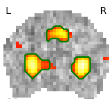
\includegraphics[width=.6\linewidth]{structure.png}
    }
\end{column}
\end{columns}

\bigskip
\bigskip
\only<3->{
  \mydot such models are more \emph{intepretable} (i.e \emph{simple} theory)
  }
\end{overlayarea}
\end{frame}

\subsection{SpaceNet}
\begin{frame}\frametitle{Regularized linear models}
  \vspace{-1.5em}
\begin{columns}
  \begin{column}{7cm}

\mydot Generalized linear model
{\huge
\[
    \tilde{\B{y}} = \B{X}\, \B{w} + \text{``error''}
\]
}%

\begin{itemize}
\item $\tilde{y}_i = \log\left(\frac{\mathbb P(y_i = +1|x_i)}{\mathbb{P}(y_i=-1|x_i)}\right)$ in \emph{classification}
\item $\tilde{y}_i = y_i$ in \emph{regression} settings
\end{itemize}

\uncover<2->{
\mydot Leads to \emph{MAP} estimation problem
}

\begin{overprint}
  \onslide<3>
  \vspace{-1em}
\begin{equation*}
\min_{\B{w} \in \mathbb R^p}\left\{E(\B{w}) := \underbrace{\ell(\B{y}, \B{Xw})}_{\text{\emph{loss}}} + \underbrace{\alpha\mathcal P(\B{w})}_{\emph{penalty}}\right\}
\end{equation*}


\onslide<4>
\mydot \emph{$\ell(\B{y},\B{X}\B{w})$} is the loss function. For example,
\vspace{-.5em}
\begin{equation*}
      \ell(\B{y},\B{X}\B{w}) =
  \frac{1}{n}\sum_{i=1}^n 
  % \begin{cases}\frac{1}{2}(\B{x}^T_i\B{w} - y_i)^2
  %   %= \frac{1}{2}(\B{X}^T_i\B{w} - \B{y}_i)^2
  %   ,
  %   &\mbox{ \text{ (least sq.)}}\\
    \log(1+\exp(-{y}_i\B{x}_i^T\B{w})),
    % &\mbox{ \text{ {(log. reg.)}}}\\
    % (1-y_i\B{x}_i^T\B{w})_+,&\mbox{ \text{(hinge)}}\\
    % \vdots\end{cases}
  \end{equation*}

  in classification problems

\end{overprint}

\end{column}

\begin{column}{4cm}

    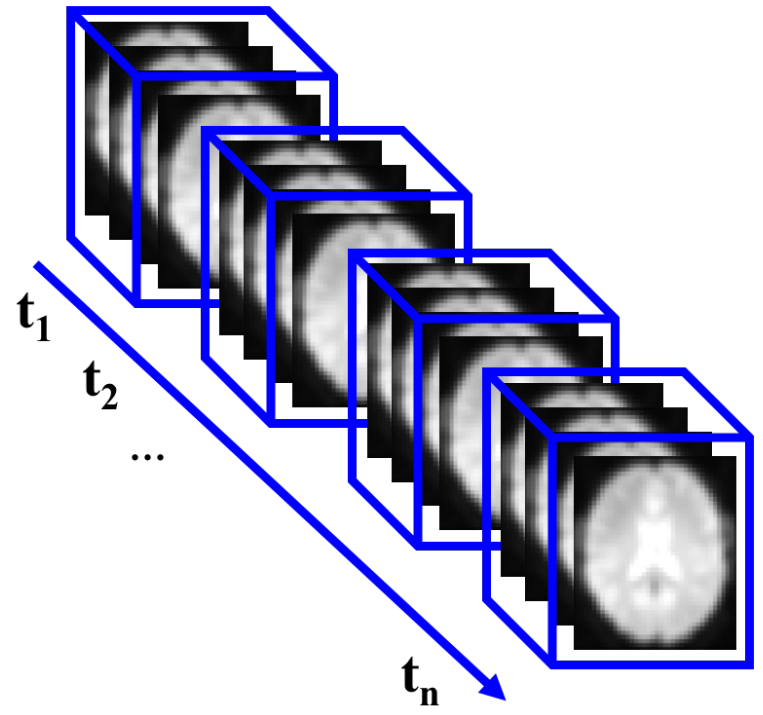
\includegraphics[width=.8\linewidth]{X.png}

    % \quad\quad\quad\quad$\B{X}$

    % \bigskip
    
    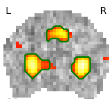
\includegraphics[width=.5\linewidth]{structure.png}

    % \quad\quad\quad\quad$\B{w}$

    \bigskip
    
    
\includegraphics[width=.4\linewidth]{cat.png}

    % \quad\quad\quad\quad$\B{w}$

\end{column}

\end{columns}
% \mydot \textcolor{green}{{$\ell(\B{y}, \B{X} \B{w})$}} is the
% \emph{loss} term
%   $$
%   \ell(\B{y},\B{X}\B{w}) =
%   \frac{1}{n}\sum_{i=1}^n 
%   \begin{cases}\frac{1}{2}(\B{x}^T_i\B{w} - y_i)^2
%     %= \frac{1}{2}(\B{X}^T_i\B{w} - \B{y}_i)^2
%     ,
%     &\mbox{ \text{ (least sq.)}}\\
%     \log(1+\exp(-{y}_i\B{x}_i^T\B{w})),
%     &\mbox{ \text{ {(log. reg.)}}}\\
%     % (1-y_i\B{x}_i^T\B{w})_+,&\mbox{ \text{(hinge)}}\\
%     \vdots\end{cases}
%   $$

\end{frame} %--------------------------------------------------------------}}}

\begin{frame}\frametitle{Zoom on the penalty}
  \begin{columns}
    \begin{column}{4cm}
      $\min_{\B{w} \in \mathbb R^p}\underbrace{\ell(\B{y}, \B{Xw})}_{\text{{loss}}} + \underbrace{\alpha\mathcal P(\B{w})}_{\emph{penalty}}$
    \end{column}
    \begin{column}{6cm}
      \only<2->{
        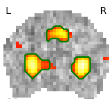
\includegraphics[width=.4\linewidth]{structure.png}
        }
        \hspace{.5em}
\uncover<5->{        
  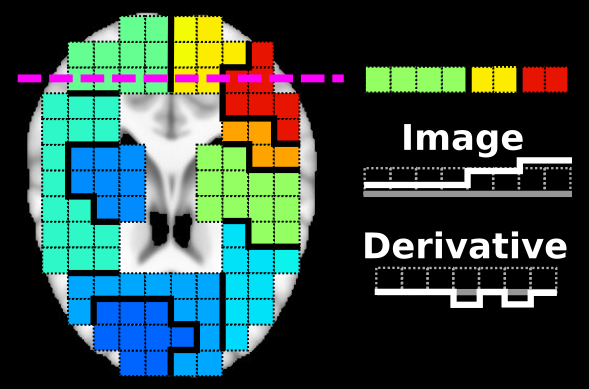
\includegraphics[width=.5\linewidth]{cartoon}
  }
    \end{column}
  \end{columns}

  \uncover<3->{
    \begin{equation*}
      \begin{split}
        \mathcal P(\B{w}) = \begin{cases}
          % \rho\|\B{w}\|_1 + \frac{1}{2}(1-\rho)\|\nabla \B{w}\|_{\text{Fro}}^2 =
          \sum_{j \in [\![p]\!]}\rho|\B{w}_j| + \frac{1}{2}(1-\rho)\|(\nabla \B{w})_j\|_2^2, &\mbox{ for GraphNet
            % ~\citep{grosenick2013,hebiri2011}
          }\\
    % \|\nabla_\rho \B{w}\|_{1+2,1} =
    % \rho\|\B{w}\|_1 + \|\nabla \B{w}\|_{2,1} =
    % \sum_{j  \in [\![p]\!]}\rho|\B{w}_j| + (1-\rho)\|(\nabla \B{w})_j\|_2, &\mbox{ for isotropic TV-$\ell_1$
    % ~\citep{baldassarre2012,gramfort2013}
  % }\\
    % \|\nabla_\rho \B{w}\|_{1,1} =
    % \rho\|\B{w}\|_1 + (1-\rho)\|\nabla \B{w}\|_{1,1} =
    \sum_{j  \in [\![p]\!]}\rho|\B{w}_j| + (1-\rho)\|(\nabla \B{w})_j\|_1, &\mbox{ for anisotropic TV-$\ell_1$
    }\\
    % \|\nabla_\rho \B{w}\|_{2,1} =
    \sum_{j  \in [\![p]\!]}\|(\nabla_\rho \B{w})_j\|_2, &\mbox{ for Sparse Variation
      %~\citep{eickenberg2015total}
    }\\
      \vdots
    \end{cases}
  \end{split}
  \label{eq:penalty}
\end{equation*}
}

\uncover<5->{
 \mydot {Bayesian view}
 \begin{eqnarray*}
   \begin{split}
     \underbrace{P(\B{w} | \B{X},\B{y})}_{\text{\emph{posterior}}} &\propto \underbrace{P(\B{y}|\B{X},\B{w})}_{\text{\emph{likelihood}}} \times \underbrace{P(\B{w})}_{\text{\emph{prior}}}
     = \exp(-\ell(\B{y},\B{X}\B{w})) \times \exp(-\alpha\mathcal P(\B{w}))
   \end{split}
 \end{eqnarray*}
}

\end{frame}

\subsection{Better but more difficult}
\begin{frame}
\frametitle{More intepretable models}
% Faces vs objects classification on \textcolor{myblue}{[Haxby 2001]}
\vspace{-2em}
\begin{overlayarea}{\textwidth}{\textheight}
\begin{columns}
  \column{.45\linewidth}
  \begin{figure}
    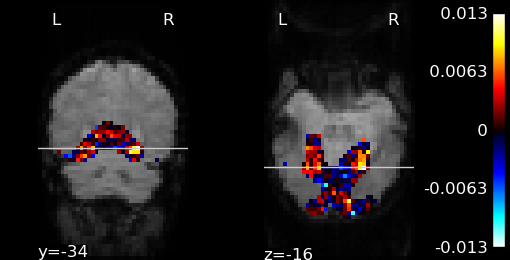
\includegraphics[width=\textwidth]{haxby_face-house_svc_weights.png}
    \caption{SVM weights}
  \end{figure}
\end{columns}

\begin{columns}
  \column{.45\linewidth}
    \only<2->{
      \begin{figure}
        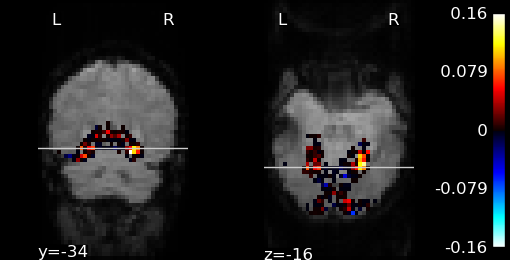
\includegraphics[width=\textwidth]{haxby_face-house_smooth-lasso_weights.png}
        \caption{S-Lasso / GraphNet}
      \end{figure}
    }

  \column{.45\linewidth}
    \only<3->{
      \begin{figure}
        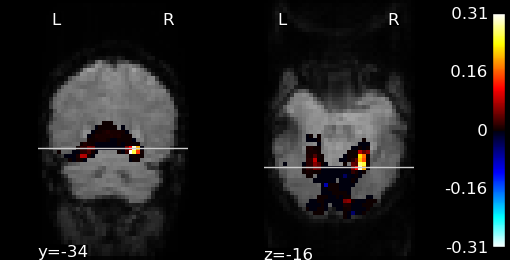
\includegraphics[width=\textwidth]{haxby_face-house_tv-l1_weights.png}
        \caption{TV-L1 weights}
      \end{figure}
      }
\end{columns}
\end{overlayarea}

\end{frame}

\begin{frame}
  \frametitle{... but much harder optimization problems!}
  \uncover<1->{
    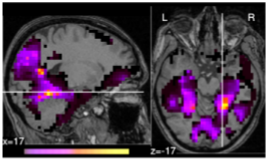
\includegraphics[width=.31\linewidth]{01.png}%
    \llap{\color{white}\raisebox{.15\linewidth}{\rlap{\sffamily
          $\Delta E < 10^{-1}$}}\hspace*{.31\linewidth}}\hfill%
  }
  \uncover<3->{
    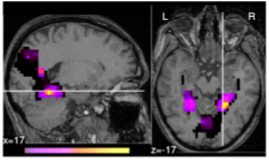
\includegraphics[width=.31\linewidth]{001.png}%
    \llap{\color{white}\raisebox{.15\linewidth}{\rlap{\sffamily
          $\Delta E < 10^{-3}$}}\hspace*{.31\linewidth}}\hfill%
  }
  \uncover<4->{
    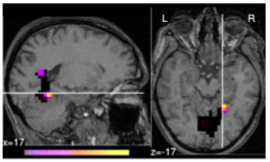
\includegraphics[width=.31\linewidth]{00001.png}%
    \llap{\color{white}\raisebox{.15\linewidth}{\rlap{\sffamily
          $\Delta E < 10^{-5}$}}\hspace*{.31\linewidth}}%
    }

\bigskip

\uncover<4->{
  \mydot Structured penalties lead to \emph{more intepretable models}
}

\bigskip

\uncover<5->{
  \mydot But corresponding optimization problem is much \emph{harder}
  \begin{itemize}
    \item \emph{high-dimensional non-smooth ill-conditioned} problem
    \item Can't compute \emph{prox operator} analytically
  \end{itemize}
}

\bigskip

\uncover<6->{
\mydot Lack of fast solver can lead to \emph{wrong conclusions about model}
}

\bigskip

\uncover<7->{
  \mydot We need \emph{fast solvers!}
}
\end{frame}

\subsection{Algorithms}
\begin{frame}
  \frametitle{Looking for the ideal solver}
  % \vspace{-.5em}
  \mycite{Dohmatob '14, '15 (PRNI); Varoquaux '15 (Gretsy)}
  % \vspace{-.5em}

  \begin{overlayarea}{\textwidth}{\textheight}
    \only<1>{
      \begin{figure}
        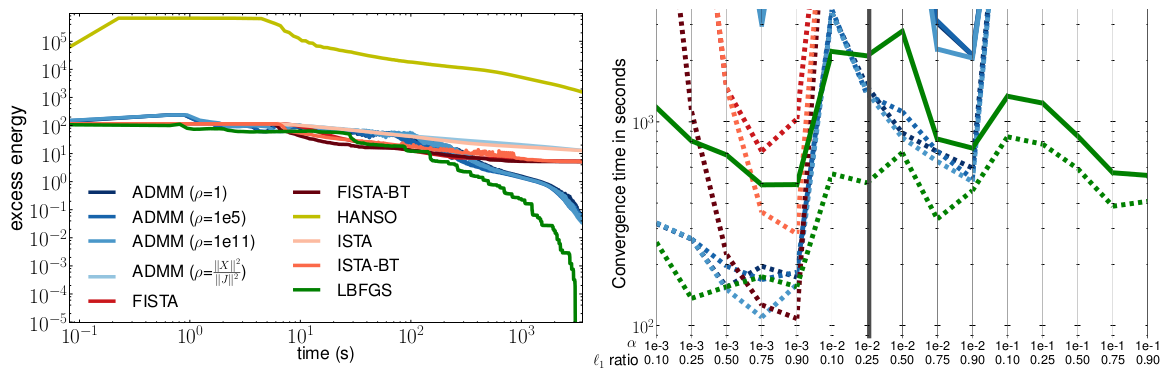
\includegraphics[width=1.05\linewidth]{figures/solvers_1.png}
        \caption{Classification: visual recognition task}
      \end{figure}
    }
    \only<2->{
      \begin{figure}
        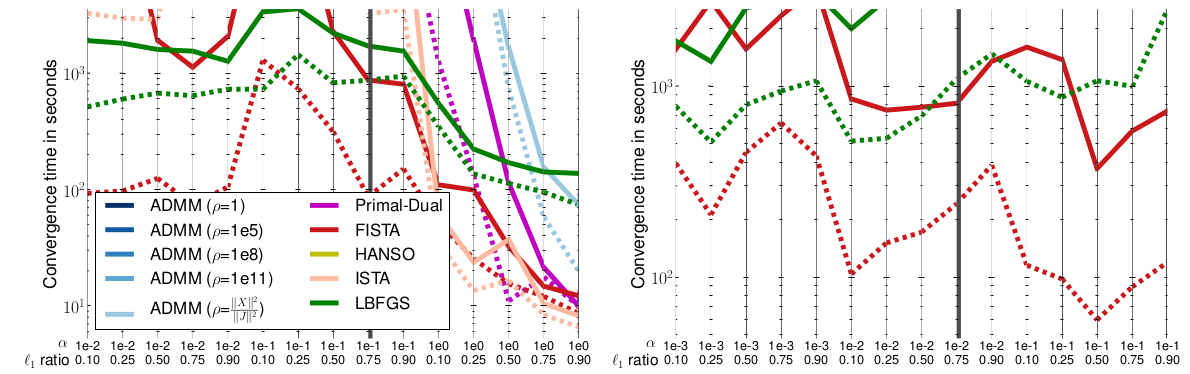
\includegraphics[width=1.05\linewidth]{figures/solvers_2.png}
        \caption{Regression: mixed-gambles}
      \end{figure}
    }
  \end{overlayarea}
\end{frame}

\begin{frame}\frametitle{More speed via univariate feature-screening}
  \vspace{-.7em}
  \mycite{Dohmatob '15 (PRNI)}
  \medskip
  
  \mydot \emph{$t_k$} := $k$th percentile of the vector $|\B{X}^T\B{y}| := (|\B{x}_1^T\B{y}|,\ldots,|\B{x}_p^T\B{y}|)$.
  
  \mydot Discard $j$th voxel if \emph{$|\B{x}^T_j\B{y}| < t_k$}
  \bigskip
  
  \quad\textcolor{blue}{$k = 10\%$}\quad\quad\quad\;\textcolor{blue}{$k = 20\%$}\quad\quad\quad\textcolor{blue}{$k = 50\%$}\quad\quad\quad\textcolor{blue}{$k = 100\%$}
  \begin{overlayarea}{\textwidth}{\textheight}
    \only<1>{
    \begin{figure}
      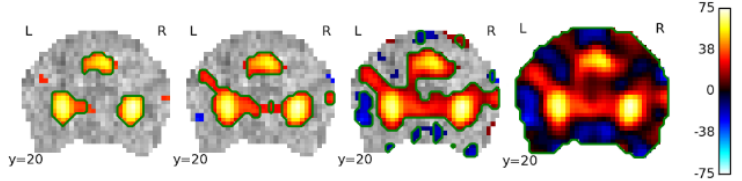
\includegraphics[width=\linewidth]{screening_gambling.png}
      \caption{Mixed gambling}
    \end{figure}
  }
  \only<2>{
    \vspace{-1em}
    \begin{figure}
      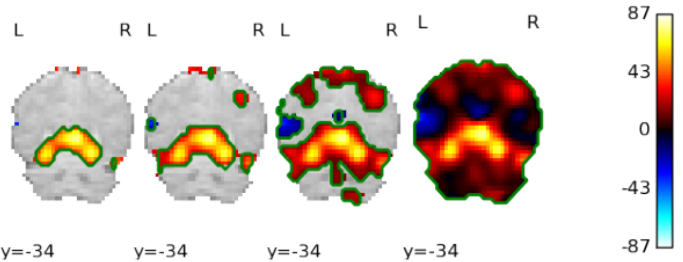
\includegraphics[width=\linewidth]{screening_haxby.png}
      \caption{Visual recognition}
    \end{figure}
  }

  \only<3>{
    \begin{figure}
      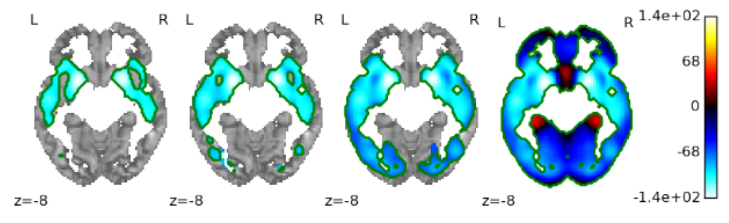
\includegraphics[width=\linewidth]{screening_oasis.png}
      \caption{Age prediction from gray-matter maps}
    \end{figure}
  }
  \end{overlayarea}

% \mydot Marginal screening \textcolor{myblue}{[Lee 2014]}, but \textcolor{red}{without} the
% (invertibility) restriction \emph{$k \le min(n, p)$}.

\end{frame}

\begin{frame}\frametitle{More speed via univariate feature-screening: results}
  \vspace{-1.1em}
  \begin{columns}
    \column{.6\linewidth}
    \begin{overlayarea}{\textwidth}{\textheight}
      \only<1>{
        \begin{figure}
          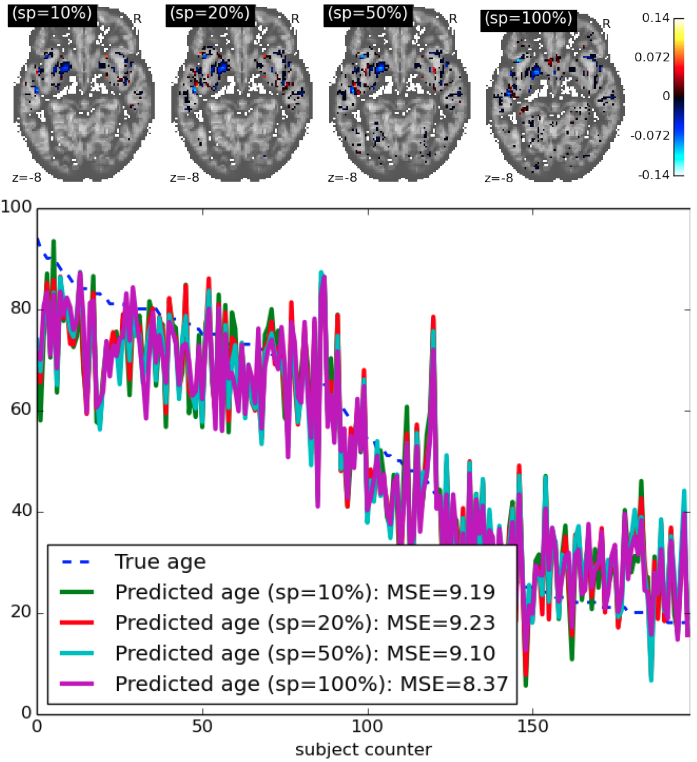
\includegraphics[width=1\linewidth]{figures/screening_oasis.png}
        \end{figure}
      }
      \only<2->{
        \begin{figure}
          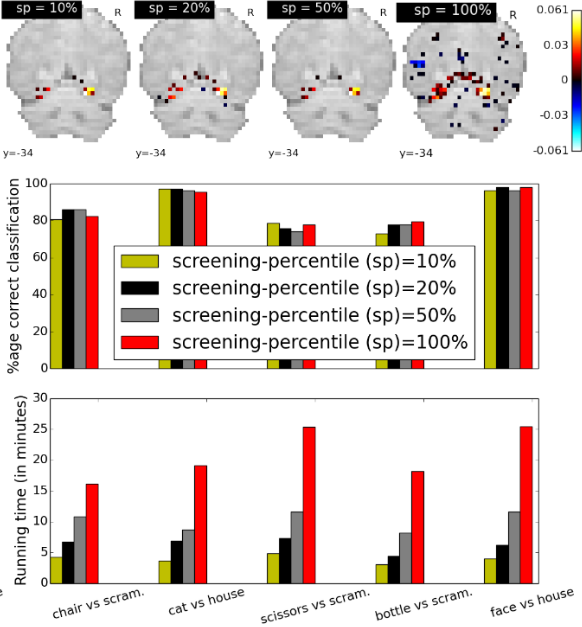
\includegraphics[width=1\linewidth]{figures/haxby_sp.png}
        \end{figure}
      }      
    \end{overlayarea}
    \column{.45\linewidth}
    \mycite{Dohmatob '15 (PRNI)}
    \bigskip
    
    % \mydot True model support approximated by screening procedure

    \mydot Solve on subset of features
    
    \bigskip
    
    \mydot Reduced training time

    \bigskip
    
    \mydot ...
  \end{columns}
 
\end{frame}


\begin{frame}\frametitle{Early-stopping}
  \begin{columns}
    \column{.7\linewidth}
    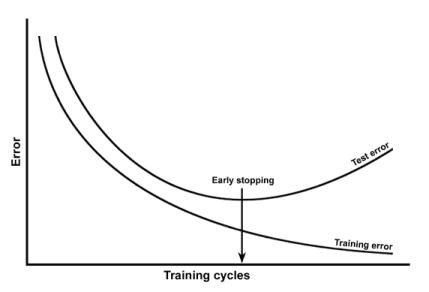
\includegraphics[width=1\linewidth]{early-stopping-graphic}
    \column{.45\linewidth}
    \mydot Old idea (e.g \mycite{Bottou})

    \bigskip
    
    \mydot Saves training time
    \bigskip
    
    \mydot implicit regularization

    \bigskip

    \mydot helps against overfitting
  \end{columns}
\end{frame}

\begin{frame}\frametitle{Early-stopping: results}
  \vspace{-1.1em}
  \begin{columns}
    \column{.6\linewidth}
    \begin{overlayarea}{\textwidth}{\textheight}
      \only<1>{
        \begin{figure}
          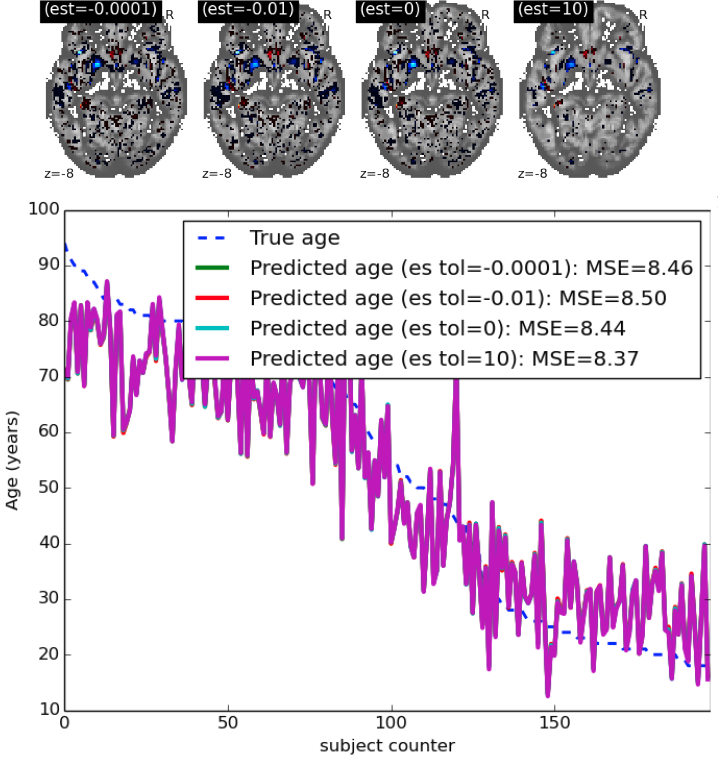
\includegraphics[width=1\linewidth]{figures/es_oasis.png}
        \end{figure}
      }
      \only<2->{
        \begin{figure}
          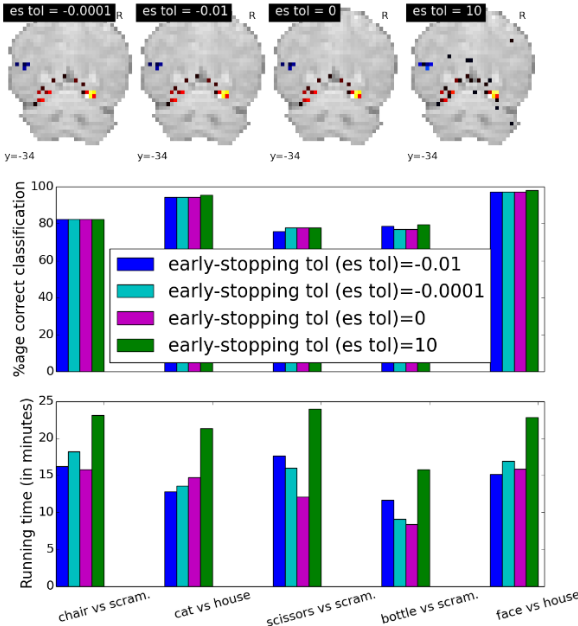
\includegraphics[width=1\linewidth]{figures/haxby_es.png}
        \end{figure}
      }      
    \end{overlayarea}
    \column{.45\linewidth}
    \mycite{Dohmatob '15 (PRNI)}
    \bigskip
    
    % \mydot True model support approximated by screening procedure

        \mydot Solve on subset of features

        \bigskip 
    \mydot Yields upto \emph{x10 speedup!}

    \bigskip
    
    \mydot No significant loss in accuracy
  \end{columns}
 
\end{frame}

% \begin{frame}\frametitle{All good, but we need fast solvers}\Large
%  \mydot Total-Variation (TV) \mycite{Michel '11},

%  \mydot S-Lasso / GraphNet \mycite{Hebiri '11, Grosenick
%      '13},

%    \mydot TV-L1 \textcolor{myblue}{[Baldassare '12, Gramfort '13]}

%  \mydot Sparse-Variation \textcolor{myblue}{[Eickenberg '15]}.

%  \mydot Algorithmics of TV-L1, GraphNet, etc.
%   \textcolor{myblue}{[Dohmatob '14, '15, Varoquaux '15]}.

%   \bigskip
  
%   \hrule

%     \bigskip

%   \mydot 
% \end{frame}

\section{Modelling inter-subject variability via dictionary-learning}
\begin{frame}
  \frametitle{Learn latent model for inter-subject variability}
  
    \mydot \emph{Goal:} Summarize inter-subject variability into a latent dimensions
    \begin{equation*}
      \begin{split}
      \B{X} &= \B{D} \times \B{C}\\
      {\includegraphics[width=.45\linewidth, valign=c]{acti.pdf}} &= {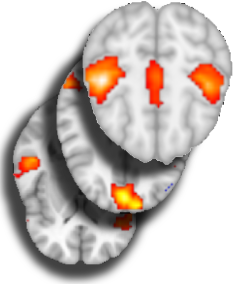
\includegraphics[width=.25\linewidth, valign=c]{dico.pdf}^T} \times \;{\includegraphics[width=.28\linewidth, valign=c]{tab.pdf}}
      \end{split}
    \end{equation*}

    \mydot $\mathbb R^p \ni \B{x}_s \overset{\B{D}}{\longrightarrow} \B{c}_s \in \mathbb R^k$, with $k \ll p$
\end{frame}  


\begin{frame}
  \frametitle{\emph{The challenge}}\Large
  \bigskip
  \bigskip
  \mydot \textcolor{red}{Sparsity:} spatially localized atoms

  \bigskip

  \mydot \textcolor{red}{Spatial blobs:} each atom = intepretable blobs

  \bigskip
  
  \mydot \textcolor{red}{Scalable / online:} model should trainable online
  \begin{itemize}
  \item scales increasing data
  \end{itemize}
  
\end{frame}


\subsection{Introducing the proposed model}
\begin{frame}
  \frametitle{Introducing the proposed model}
  \vspace{-2em}
    \begin{equation*}
      \begin{split}
      {\includegraphics[width=.45\linewidth, valign=c]{acti.pdf}} &= {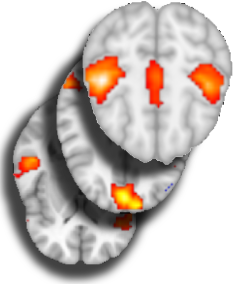
\includegraphics[width=.25\linewidth, valign=c]{dico.pdf}^T} \times \;{\includegraphics[width=.28\linewidth, valign=c]{tab.pdf}}
      \end{split}
    \end{equation*}
\vspace{-1.5em}
\begin{eqnarray*}
  \begin{split}
    &\min_{\B{D} \in \mathbb R^{p \times k}}\left(\lim_{n \rightarrow \infty}\frac{1}{n}\sum_{t=1}^n\min_{\B{c}_t \in \mathbb R^{k}}\frac{1}{2} \|\B{x}_t-\B{D}\B{c}_t\|_2^2 +  \frac{1}{2}\alpha\|\B{c}_t\|_2^2\right) + \textcolor{orange}{\gamma\sum_{j=1}^k\Omega_{\text{Lap}}(\B{d}^j)},\\
    &\textcolor{orange}{\text{subject to } \B{d}^1,\ldots,\B{d}^k \in \mathcal K}
  \end{split}
\end{eqnarray*}

% \emph{\textbf{N.B.:}} You may see this a s kind of online PCA with structural constraints on the components / atoms.

\uncover<2-> {
  \mydot $\mathcal K \subseteq \mathbb R^p$ is an $\ell_1$ ball

  \mydot $\Omega_{\text{Lap}}(\B{d}) := \frac{1}{2}\|\nabla \B{d}\|_F^2$, penalty that \emph{imposes blobs} in atoms $\B{d}$.
}

\end{frame}


\subsection{Algorithms}
\begin{frame}
  \frametitle{Putting everything together: The Algorithm}
  \rlap{\smash{
\includegraphics[width=1.5em]{loop}}}%
  \vspace{-1em}
  \begin{itemize}
\uncover<2->{    
\item \emph{Draw a sample} 3D brain image $\B{x}_t \in \mathbb R^p$
}
\uncover<3->{
  \item \emph{Compute code} (i.e representation w.r.t current dictionary $\B{D}$)
    \begin{equation*}
      \B{c}_t \leftarrow \argmin_{\B{u} \in \mathbb R^k}\frac{1}{2}\|\B{x}_t -
      \B{D} \B{u}\|_2^2 + \frac{1}{2}\alpha\|\B{u}\|_2^2.
    \end{equation*}
  \item \emph{Rank-1 }updates: $\B{A}_t = \B{A}_{t-1} + \B{c}_t\B{c}_t^T$, $\B{B}_t := \B{B}_{t-1} + \B{x}_t\B{c}_t^T$
}
    \uncover<4->{
    
  \item \emph{BCD dictionary update }of dictionary atoms

    \mydot \emph{Precompute} $\B{R} \leftarrow \B{B} - \B{D}\B{A}$

    \mydot
    \vspace*{.5em}
    \hspace{.1em}\rlap{\smash{
\includegraphics[width=1em]{loop}}}%
    \quad\emph{ for} $j = 1,2,\ldots,k$
    
    % \quad\quad\quad\emph{\# Update} $j$th atom of dictionary % (few FISTA iters.)

    \quad\quad\quad\mydot \emph{Rank-1 }update: $\B{R} \leftarrow \B{R} + \B{d}^j \circ \B{a}^j$
    
    \quad\quad\quad\mydot \emph{FISTA loop: } $\B{d}^j \leftarrow
    \argmin_{\B{d} \in \mathcal K}F_{\gamma_t}(\B{d}, a_{j,j}^{-1}\B{r}^j)
    % = \prox_{(\textcolor{red}{F_{\gamma_t} + i_{\mathcal K}})}(a_{j,j}^{-1}\B{r}^j)
    $

    \quad\quad\quad\mydot \emph{Rank-1 }update: $\B{R} \leftarrow \B{R} - \B{d}^j \circ \B{a}^j$
  }    
\end{itemize}
  \hrule
  \bigskip

  \uncover<5->{
  \mydot \emph{N.B.:} $F_{\gamma_t}(\B{d},\B{z}) := \frac{1}{2}\|\B{d} - \B{z}\|_2^2
  + \frac{1}{2}\gamma_t\|\nabla\B{d}\|_{\text{F}}^2$, $\gamma_t := \gamma (a_{j,j}/t)^{-1}$

  }
  
\end{frame}

\begin{frame}
  \frametitle{{Tuning the model's hyper-parameters}}%\Large
  \bigskip
  \bigskip
  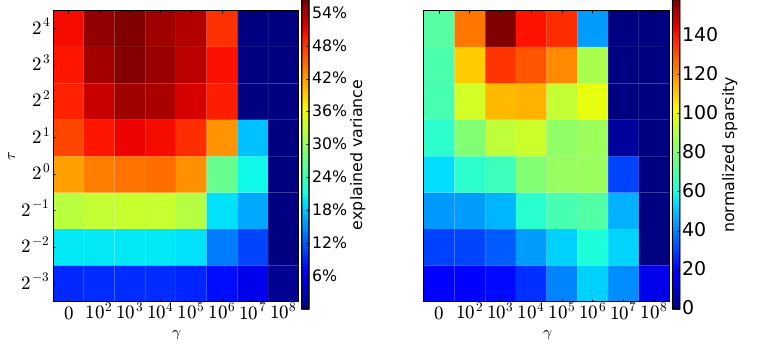
\includegraphics[width=1.\linewidth]{cv.png}
  \bigskip
  
  \mydot{The red spots are the best spots}

  \bigskip
  
  \mydot{Can be located find them via cross-validation}
\end{frame}  


% \subsection{Extension: Proximal online updates for dictionary-learning}
\begin{frame}
  \frametitle{Extension: Proximal online updates for dictionary atoms}
  \vspace{-2em}
\begin{table}[H]
  \begin{tabular}{p{3.cm}|c|p{13cm}}\hline
    \emph{penalty $g$} & \emph{$\B{p} = \prox_{\gamma g}(\B{z})$} & \emph{comments}\\\hline
    L2 ball constraint & $p_v = \B{z}_v\frac{\gamma}{\max(\gamma,\|\B{z}\|_2)}$ & \mycite{Mairal 2010}\\ \hline
%    nonneg. constraint & $p_v = (\B{z}_v)_+$ & used in NMF\\ \hline
    convex constraint & $\B{p} = \proj_{\mathcal K}(\B{z})$ & interesting for simple $\mathcal K$\\ \hline
    L1 penalty & $p_v = z_v\left(1 - \frac{\alpha}{|z_v|}\right)_+$ & soft-thresholding \\\hline
    Group L2/L1 & $\B{p}_v = \B{z}_v\left(1 - \frac{\gamma}{\|\B{z}_v\|_2}\right)_+$ & $i$ is a group of features\\\hline
    Social sparsity \newline \mycite{Kowalski '09} & $p_v = z_v\left(1 - \frac{\gamma}{\|\boldsymbol{\omega}_v * \B{z}\|_2}\right)_+$
                                                    & feature $i$ survives if avg. \newline energy in neigh. is high\\\hline
    % Social sparsity & $p_v = z_v\left(1 - \frac{\gamma}{\left(\sum_{l \in \mathcal N(i)}(\omega^{l}_{i})^2z_{l}^2\right)^{1/2}}\right)_+$
    %                                                 & denominator is just a \newline
    %                                                 convolution\\\hline
%    etc. & etc. & etc.\\\hline
  \end{tabular}
\end{table}

\vspace{-1.5em}
\begin{overlayarea}{\textwidth}{\textheight}
\begin{columns}
  \column{.35\linewidth}
  \only<2->{
    \vspace{3.5em}
    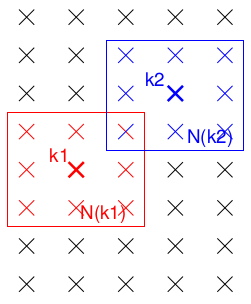
\includegraphics[width=.8\linewidth]{social.png}
  }

\vspace{-4em}  
\column{.65\linewidth}
\only<3->{
  \emph{Zoom on social sparsity }\mycite{Kowalski '09}

  \mydot $\|\boldsymbol{\omega}_v * \B{z}\|_2^2 := \sum_{l \in \mathcal N(i)}\omega^{l}_{i}z_{l}^2 \ge 0$%, a convolution with weights $\omega_v^1, \ldots,\omega_v^p \ge 0$,
%  where $\sum_{i}\omega_v^l = 1$, $\forall l \in [\![p]\!]$

  \bigskip
  
  \mydot Imposes \emph{sparsity} and \emph{smoothness}!
  }
\end{columns}
\end{overlayarea}
\end{frame}

\begin{frame}
  \frametitle{{Proximal online updates for dictionary atoms}}
  % \mydot Our proposed model can an be extended to more general structured penalties of the form \emph{$\Omega(\B{D}) := \sum_{j=1}^kg_j(\B{d}^j)$}. Viz,
  \begin{overprint}
    \onslide<1>
    \begin{eqnarray*}
      \begin{split}
        &\min_{\B{D} \in \mathbb R^{p \times k}}\frac{1}{n}\sum_{t=1}^n\left(\min_{\B{c}_t \in \mathbb R^{k}}\frac{1}{2} \|\B{x}_t-\B{D}\B{c}_t\|_2^2 +  \alpha\|\B{c}_t\|_2^2\right) + \gamma\textcolor{red}{\sum_{j=1}^k\Omega_{\text{Lap}}(\B{d}^j)}.\\
    &\textcolor{red}{\text{subject to } \B{d}^1,\ldots,\B{d}^k \in \mathcal K}
  \end{split}
    \end{eqnarray*}
\onslide<2->
\begin{eqnarray*}
  \begin{split}
&\min_{\B{D} \in \mathbb R^{p \times k}}\frac{1}{n}\sum_{t=1}^n\left(\min_{\B{c}_t \in \mathbb R^{k}}\frac{1}{2} \|\B{x}_t-\B{D}\B{c}_t\|_2^2 +  \alpha\|\B{c}_t\|_2^2\right)
     + \gamma\textcolor{green}{\sum_{j=1}^kg_j(\B{d}^j)}.
   \end{split}
\end{eqnarray*}
\end{overprint}

% \mydot Here, the \emph{$g_j$}'s are \textit{proximable} (e.g group-Lasso, social sparsity)
% \bigskip
\uncover<3->{
\textbf{\textcolor{orange}{The proximal online BCD updates:}}\\
\begin{equation*}
  \begin{split}
    \vspace*{-1em}
    \rlap{\smash{
\includegraphics[width=2em]{loop}}}%      
    \quad\quad\B{d}^j \leftarrow \prox_{\gamma a_{j,j}^{-1}g_j}(\B{z}^{-j}),\;j \leftarrow j + 1 \text{ (go to next atom)}
  \end{split}
  \end{equation*}
\mydot $\B{z}^{-j} := a_{j,j}^{-1}\B{r}^j$ and $\B{R} := \left(\B{b}^j-\sum\nolimits_{l \ne j}a_{j,l}\B{d}^l\right) = \B{B}- \B{DA} + \B{d}^j \circ \B{a}^j $.
}

\uncover<4->
{
  \mydot \emph{Bonus:} It suffices to specify the $g_j$'s only via their prox!
\begin{itemize}
\item E.g Social sparsity! \mycite{Kowalski '09}
\end{itemize}
}

\end{frame}


\subsection{Results}
\begin{frame}
  \frametitle{Experimental on results HCP fMRI data: qualitative}
  \begin{overlayarea}{\textwidth}{\textheight}
  \only<1->{
    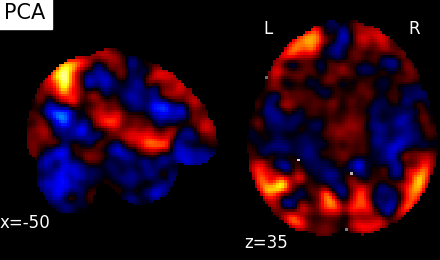
\includegraphics[width=0.32\linewidth]{{figures/components_LANGUAGE_nc=40_PCA_7}.png}
  }
  \only<2->{
    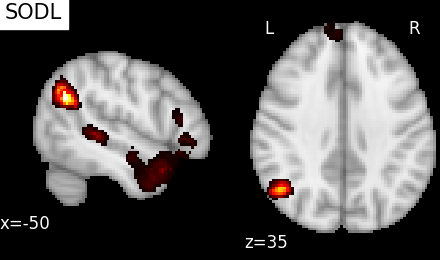
\includegraphics[width=0.32\linewidth]{{figures/components_LANGUAGE_nc=40_alpha=auto_gamma=0_radius=4_split=0_time=12_29}.png}
  }
  \only<3->{
  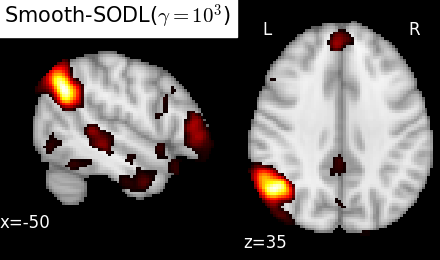
\includegraphics[width=0.32\linewidth]{{figures/components_LANGUAGE_nc=40_alpha=auto_gamma=1000_radius=4_split=0_time=12_29}.png}
}
\only<4->{
    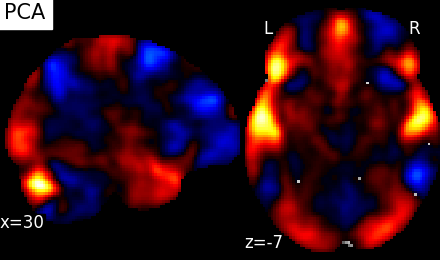
\includegraphics[width=0.32\linewidth]{{figures/components_LANGUAGE_nc=40_PCA_1}.png}
  }
  \only<5->{
    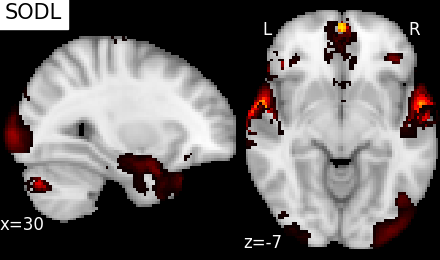
\includegraphics[width=0.32\linewidth]{{figures/components_LANGUAGE_nc=40_alpha=auto_gamma=0_radius=4_split=0_time=12_37}.png}
  }
  \only<6->{
    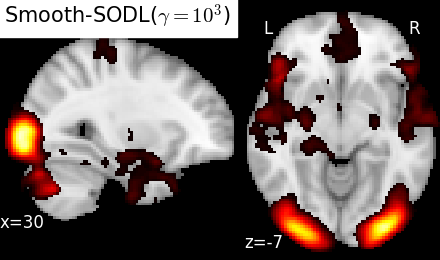
\includegraphics[width=0.32\linewidth]{{figures/components_LANGUAGE_nc=40_alpha=auto_gamma=1000_radius=4_split=0_time=12_36}.png}
  }
\only<7->{
    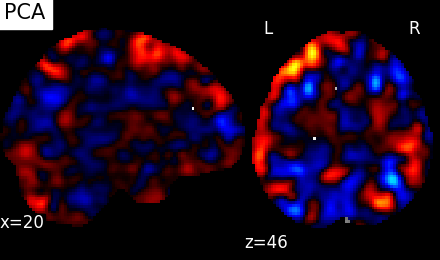
\includegraphics[width=0.32\linewidth]{{figures/components_LANGUAGE_nc=40_PCA_33}.png}
  }
  \only<8->{
    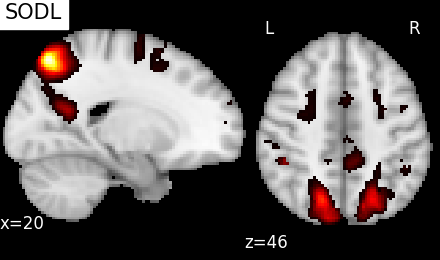
\includegraphics[width=0.32\linewidth]{{figures/components_LANGUAGE_nc=40_alpha=auto_gamma=0_radius=4_split=0_time=12_22}.png}
  }
  \only<9->{
    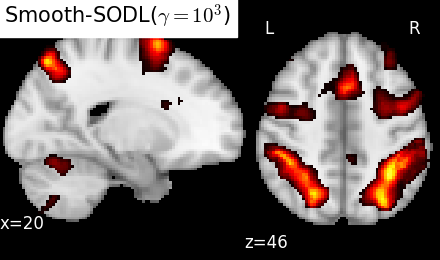
\includegraphics[width=0.32\linewidth]{{figures/components_LANGUAGE_nc=40_alpha=auto_gamma=1000_radius=4_split=0_time=12_4}.png}
    }  
\end{overlayarea}
  
% 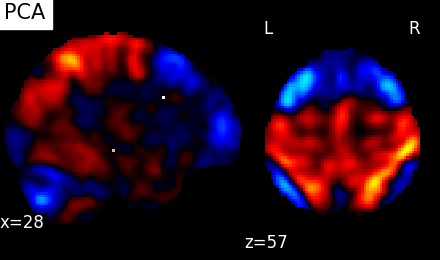
\includegraphics[width=0.2\linewidth]{{figures/components_LANGUAGE_nc=40_PCA_2}.png}
% 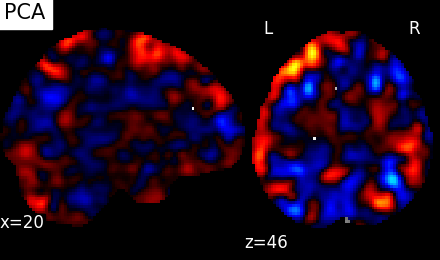
\includegraphics[width=0.2\linewidth]{{figures/components_LANGUAGE_nc=40_PCA_33}.png}
% 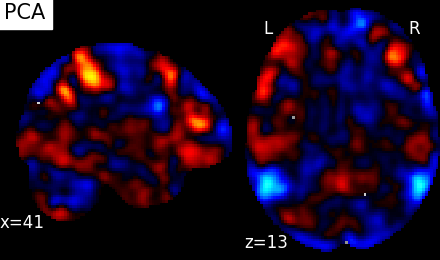
\includegraphics[width=0.2\linewidth]{{figures/components_LANGUAGE_nc=40_PCA_25}.png}
% \includegraphics[width=0.2\linewidth]{{figures/components_LANGUAGE_nc=40_PCA_7}.png}
% \includegraphics[width=0.2\linewidth]{{figures/components_LANGUAGE_nc=40_PCA_1}.png}
% \\
% \includegraphics[width=0.2\linewidth]{{figures/components_LANGUAGE_nc=40_alpha=auto_gamma=0_radius=4_split=0_time=12_34}.png}
% \includegraphics[width=0.2\linewidth]{{figures/components_LANGUAGE_nc=40_alpha=auto_gamma=0_radius=4_split=0_time=12_22}.png}
% \includegraphics[width=0.2\linewidth]{{figures/components_LANGUAGE_nc=40_alpha=auto_gamma=0_radius=4_split=0_time=12_4}.png}
% \includegraphics[width=0.2\linewidth]{{figures/components_LANGUAGE_nc=40_alpha=auto_gamma=0_radius=4_split=0_time=12_29}.png}
% \includegraphics[width=0.2\linewidth]{{figures/components_LANGUAGE_nc=40_alpha=auto_gamma=0_radius=4_split=0_time=12_37}.png}
% \\
% \includegraphics[width=0.2\linewidth]{{figures/components_LANGUAGE_nc=40_alpha=auto_gamma=1000_radius=4_split=0_time=12_3}.png}
%   \includegraphics[width=0.2\linewidth]{{figures/components_LANGUAGE_nc=40_alpha=auto_gamma=1000_radius=4_split=0_time=12_4}.png}
% \includegraphics[width=0.2\linewidth]{{figures/components_LANGUAGE_nc=40_alpha=auto_gamma=1000_radius=4_split=0_time=12_8}.png}
% \includegraphics[width=0.2\linewidth]{{figures/components_LANGUAGE_nc=40_alpha=auto_gamma=1000_radius=4_split=0_time=12_29}.png}
% \includegraphics[width=0.2\linewidth]{{figures/components_LANGUAGE_nc=40_alpha=auto_gamma=1000_radius=4_split=0_time=12_36}.png}

% \\
% \includegraphics[width=0.2\linewidth]{{figures/components_LANGUAGE_nc=40_CanICA_26}.png}
% \includegraphics[width=0.2\linewidth]{{figures/components_LANGUAGE_nc=40_CanICA_9}.png}
% \includegraphics[width=0.2\linewidth]{{figures/components_LANGUAGE_nc=40_CanICA_31}.png}
% \includegraphics[width=0.2\linewidth]{{figures/components_LANGUAGE_nc=40_CanICA_28}.png}
% \includegraphics[width=0.2\linewidth]{{figures/components_LANGUAGE_nc=40_CanICA_23}.png}
% \\
% \includegraphics[width=0.2\linewidth]{{figures/components_LANGUAGE_nc=40_tCanICA_26}.png}
% \includegraphics[width=0.2\linewidth]{{figures/components_LANGUAGE_nc=40_tCanICA_9}.png}
% \includegraphics[width=0.2\linewidth]{{figures/components_LANGUAGE_nc=40_tCanICA_31}.png}
% \includegraphics[width=0.2\linewidth]{{figures/components_LANGUAGE_nc=40_tCanICA_28}.png}
% \includegraphics[width=0.2\linewidth]{{figures/components_LANGUAGE_nc=40_tCanICA_23}.png}

% \mydot Each column represents an atom of the estimated dictionary
%% , where atoms from
%%   the different models (the rows of the plots) have been matched via a Hungarian algorithm. Here, we only show a limited number of the most ``intepretable'' atoms.

\mydot Our method (Smooth-SODL) produces \emph{the coolest brain maps!}
%% We see that our proposed approach produces more structured dictionaries: the atoms are well-segmented piece-wise smooth and compact, making up blobs, as opposed to scattered patterns of activation.

% \mydot  Maps corresponding to hard-thresholded CanICA
% \mycite{Varoquaux 2010} components have also been included, and have been called tCanICA.
% In contrast, the maps from vanilla \mycite{Mairal 2010} and our proposed method were not been thresholded.
\end{frame}

\begin{frame}
  \frametitle{Experimental results on HCP fMRI data: quantitative}
  \includegraphics[width=.36\linewidth]{figures/ev_scores_LANGUAGE.pdf}
%  \hspace{.05cm}
  \includegraphics[width=.7\linewidth]{figures/behavioral_scores_LANGUAGE.pdf}
  \bigskip

  \mydot \textbf{Left:} Mean explained variance of dictionary atoms
  
  \mydot \textbf{Right:} Predicting  behavioral  from language activation.
  
  \mydot Thick bars $\implies$ scores on \emph{train}; faint bars $\implies$ scores on \emph{test}


  % \bigskip
  % %\textbf{N.B.:} Bold bars represent performance on \textbf{test} set while faint bars in the 
  %  % background represent performance on \textbf{train} set.
\end{frame}

\begin{frame}
  \frametitle{Do we really need spatial regularization ?}
  \begin{overlayarea}{\textwidth}{\textheight}  
\uncover<1->{  
\mydot Answer: \emph{Yes}, it reduces sample-complexity!
  }

  \only<2->{
\begin{table}[H]
  \begin{tabular}{|c|c|c|c|c}\hline%\hline
    {Nb. subjects} & {vanilla \mycite{Mairal '10}} & {proposed model} & {gain factor} \\ \hline
17 & {2\%} & \emph{31\%} & \emph{13.8}\\\hline
92 & 37\% & \emph{50\%} & \emph{1.35}\\\hline
167 & 47\% & \emph{54\%} & \emph{1.15}\\\hline
241 & 49\% & \emph{55\%} & \emph{1.11}\\ \hline
  \end{tabular}
  \vspace{.5em}
  \caption{\textbf{Learning-curve} for ``boost'' in explained variance of our proposed Smooth-SODL model over
    the reference SODL model.
    % Note the reduction in the explained variance gain as more data are pooled.
  }
  \label{table:ev}
\end{table}
}
\end{overlayarea}
\end{frame}

\begin{frame}
  \frametitle{{Wrap-up}}%\Large
  \mydot Encoding model for \emph{inter-subject functional variability}

  \bigskip

  \mydot Encompasses \emph{known neuro-biological priors} about brain activity
  \begin{itemize}
    \item \emph{localized blobs}
  \end{itemize}

  \bigskip

  \mydot \emph{Scales} to small, medium, and large-data regimes alike
  
% \mydot To extract structured functionally discriminating patterns
% from \emph{massive brain data} (i.e data-driven atlases), we have extended
% the \emph{online dictionary-learning} \mycite{Mairal 2010}, to learn \emph{structured regions}
%  representative of brain organization.
%  \bigskip
 
% \mydot Experiments show that the proposed model %--Smooth-SODL model--
% extracts structured and \emph{denoised dictionaries} that are more \emph{intepretable} and better
% capture \emph{inter-subject variability} in small medium, and large-scale regimes alike,
% compared to state-of-the-art models.
\end{frame}


\section{Predicting task activation from resting-state data}
\begin{frame}
  \frametitle{Can we infer these cognitive maps from resting-state data ?}
  \vspace{-2.3em}
  \begin{equation*}
    \bordermatrix{&{\textcolor{orange}{\text{activity at rest }}} \cr
      \B{X}_1 & \includegraphics[width=.25\linewidth, valign=c]{connectome.png}\cr
      % \B{X}_2 & \includegraphics[width=.2\linewidth, valign=c]{connectome.png}\cr
      \vdots &\vdots \cr
      \B{X}_N & \includegraphics[width=.25\linewidth, valign=c]{connectome.png}
      }
      \underset{\textbf{ML model}}{\includegraphics[width=.2\linewidth, valign=c]{arrow.png}}\;
    \bordermatrix{&{\textcolor{orange}{\text{cognitive maps}}} \cr
      \B{Y}_1 & \includegraphics[width=.25\linewidth, valign=c]{{cogmaps_diff}.png}
      % \hspace{-7em}\includegraphics[width=.2\linewidth, valign=c]{{cogmaps_diff}.png}
      \cr
      % \B{Y}_2 & \includegraphics[width=.2\linewidth, valign=c]{{cogmaps_diff}.png}\cr
      \vdots &\vdots \cr
      \B{Y}_N & \includegraphics[width=.25\linewidth, valign=c]{{cogmaps_diff}.png}
      }
   \end{equation*}

   \mydot $\B{X}_s$: resting-state functional connectivity graph for subject $s$
 
   \mydot $\B{Y}_s$: task-specific activation maps for subject $s$

\end{frame}

subsection{Deep semi-supervised ML}
\begin{frame}
  \frametitle{Proposal: Deep semi-supervised voxel encoding}

  \includegraphics[width=1.\linewidth]{gen_model.jpg}
  
 \mydot $\B{Y} \in \mathbb R^{p \times C}$: (GLM) maps of brain activity to $C$ different specific cognitive task contrasts

 \mydot $\B{X} \in \mathbb R^{p \times T}$: resting-state data % (subjects lying in the scanner focusing on nothing)
    
  \emph{\textbf{Goal:}}

  \quad \mydot Develop model for predicting $\B{Y}$ from $\B{X}$.

\uncover<2->{  
  \emph{\textbf{Strategy:}}

  \quad \mydot \emph{Learn unsupervised voxel encoding} $\mathbb R^T \ni \B{x} \mapsto  \phi(\B{x}) \in \mathbb R^k$.
  
  \quad\quad \mydot DL (dictionary-learning) = shared-encoder layer
  
  \quad \mydot Plug the output into a \emph{linear regressor}: $\mathbb R^C \ni \B{y} \approx \phi(\B{x})^T\B{W}$.
  }
\end{frame}


\subsection{Tables}
\begin{frame}\frametitle{Tables}
\begin{tabular}{|c|c|c|}
\hline
\textbf{Date} & \textbf{Instructor} & \textbf{Title} \\
\hline
WS 04/05 & Sascha Frank & First steps with  \LaTeX  \\
\hline
SS 05 & Sascha Frank & \LaTeX \ Course serial \\
\hline
\end{tabular}
\end{frame}


\begin{frame}\frametitle{Tables with pause}
\begin{tabular}{c c c}
A & B & C \\ 
\pause 
1 & 2 & 3 \\  
\pause 
A & B & C \\ 
\end{tabular} 
\end{frame}

\section{Concluding remarks}
\subsection{blocs}
\begin{frame}\frametitle{blocs}

\begin{block}{title of the bloc}
bloc text
\end{block}

\begin{exampleblock}{title of the bloc}
bloc text
\end{exampleblock}


\begin{alertblock}{title of the bloc}
bloc text
\end{alertblock}
\end{frame}

\subsection{Pictures} 
\begin{frame}\frametitle{pictures in latex beamer class}
  % \begin{figure}
  \centering
\includegraphics[scale=.32]{howbrainworks0} 
% \caption{show an example picture}
% \end{figure}
\end{frame}

\subsection{joining picture and lists} 

\begin{frame}
\frametitle{pictures and lists in beamer class}
\begin{columns}
\begin{column}{5cm}
\begin{itemize}
\item<1-> subject 1
\item<3-> subject 2
\item<5-> subject 3
\end{itemize}
\vspace{3cm} 
\end{column}
\begin{column}{5cm}
\begin{overprint}
\includegraphics<2>{PIC1}
\includegraphics<4>{PIC2}
\includegraphics<6>{PIC3}
\end{overprint}
\end{column}
\end{columns}
\end{frame}


\subsection{pictures which need more space} 
\begin{frame}[plain]
\frametitle{plain, or a way to get more space}
\begin{figure}
\includegraphics[scale=0.5]{PIC1} 
\caption{show an example picture}
\end{figure}
\end{frame}



\end{document}
